\documentclass{article}
\usepackage{hyperref}
\usepackage{graphicx}
\usepackage{geometry}
 \geometry{
 a4paper,
 total={170mm,257mm},
 left=30mm,
right=30mm,
 top=30mm,
bottom=15mm,
 }
\hypersetup{
    colorlinks=true,
    linkcolor=blue,
    filecolor=magenta,      
    urlcolor=cyan,
}
\setlength{\parskip}{1em}
\begin{document}
\title{GAN collections}
\author{Zhi Li}
\maketitle
\section{GAN}
\subsection{Applications}
\href{https://arxiv.org/pdf/1406.2661.pdf}{GAN} is kind-of unsupervised learning for generating sequences, graphs, videos etc. Check out all the applications here. \href{https://github.com/nashory/gans-awesome-applications}{collections of awesome GAN applications}. Gernerally, input some random noise, the model will be trying to output the data satisfying to your domain. Some interesting examples like horse to zebra, shoes transformation, and face aging animation.

Problems lies in the aera that how to transform the random input towards something meaningful. This corresponds to the data distribution transformation, which will later display in the loss function.

The philosophy behind GAN is that, we train two frameworks, one for generator which input random noise and output useful results, and the other is discriminator which will drive generator to produce good results. This
framework corresponds to a minimax two-player game. Generator will be forcing to generate something to fool discriminator while discriminator will classify the fake data.

Some related work to do so including deep-Boltzmann machine, Deep Belief Networks, Variational AutoEncoder (VAE)
\subsection{Adversarial Nets}
In his paper, he suggests that optimal Discriminator \textit{D} is achieved when \textit{G} is fixed.
\begin{figure}[h!]
\centering
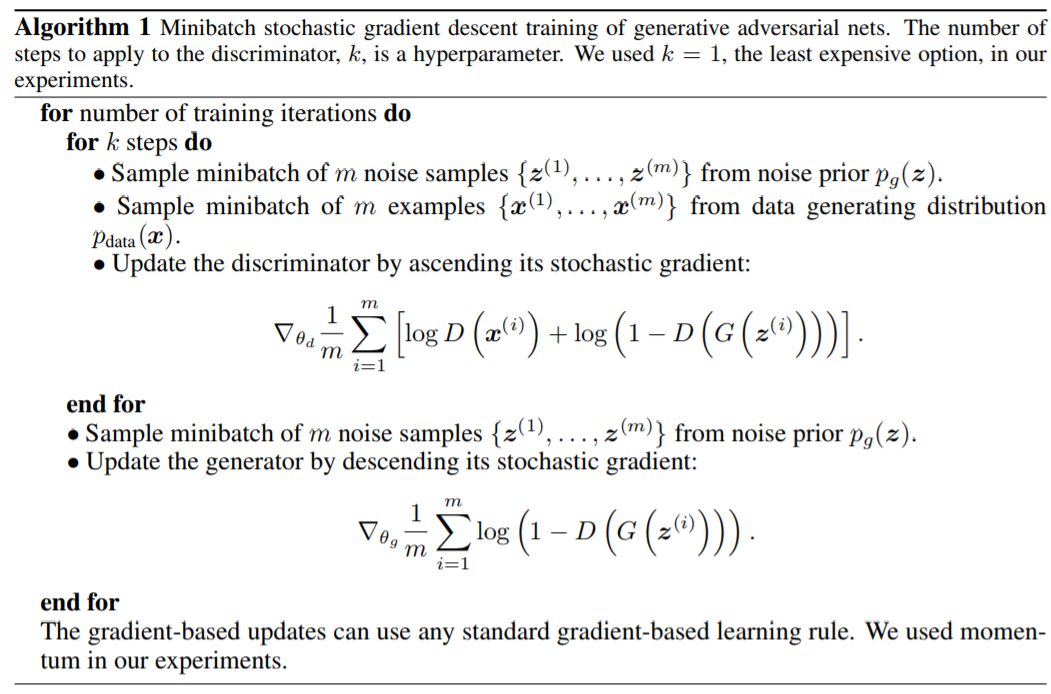
\includegraphics[width=\linewidth]{GAN-Goodfellow}
\caption{Algorithm description}
\end{figure}\\

\begin{equation}
\label{1.1}
D^{*}_{G}(x)=\frac{p_{data}(x)}{p_{data}(x)+p_g(x)} 
\end{equation}
\textbf{Theorem}. If \(p_{g}=p_{data}\) which means the global minimum. C(G) will achieve the value of $-log4$.

\section{Various GAN}
\subsection{MMGAN}
The one proposed by Goodfellow, the original loss function used for
 discriminator is $-log(1- D(x))$ (cross-entropy)

\subsection{NSGAN}
In NSGAN, the difference between it with MMGAN is that it starts to use $-log(D(x))$ because it proves that, at the begining, the gradient for $-log(1-D(x))$ is small which may not reasonable as we need the gradient to be large to converge. So with $log(D(x))$, it initialized a higher gradient at first and decreasing progressively.

\section{CGAN}
\subsection{Applications}
\subsection{Diagram}
\subsection{Loss Function}

\section{WGAN}
\subsection{Applications}

\subsection{Diagram}
\subsection{Loss Function}
\subsubsection{Generator loss}
\section{SGAN}
\subsection{Applications}
\subsection{Diagram}
\subsection{Loss Function}
\subsubsection{Generator loss}
\section{infoGAN}
\subsection{Applications}
\subsection{Diagram}
\subsection{Loss Function}
\subsubsection{Generator loss}
\section{tempoGAN}
\subsection{Applications}
\subsection{Diagram}
\subsection{Loss Function}
\subsubsection{Generator loss}
\section{Summary}
\begin{table*}[ht!]
\begin{tabular*}{\textwidth}{c @{\extracolsep{\fill}}|c|c|c}
\hline
GANS & Archive & Loss Function \\
\hline
GAN&\href{https://arxiv.org/pdf/1406.2661.pdf}{Arxiv}& $L_D^{GAN}=E[log(D(x))]+E[log(1-D(G(z))]$\linebreak$L_G^{GAN}=E[log(D(G(z)]$ \\

\hline
\end{tabular*}
\end{table*}
\end{document}
